\section{Conceptos Fundamentales de Grafos}

Partiremos nuestro estudio un par de ejemplos que sugerirán una definicón para lo que es un \emph{grafo} y motivarán el tipo de aplicaciones para los que se utilizan.
El primero que veremos se suele citar como el que dio inicio a la teoría de grafos.

\begin{ejemplo}[Los Puentes de K\"onigsberg.]
La ciudad de K\"onigsberg (hoy conocida como Kaliningrado) estaba localizada en el este de Prussia.
La ciudad tenía una isla que formaba el río Pregel al cruzarla, y antes de dejar la ciudad el río se bifurcaba dando paso a dos causes distintos.
Las regiones formadas por el río estaban unidas con siete puentes.
Un diagrama simplificado de la ciudad puede verse en la figura~\ref{fig:konigsberg}.

\begin{figure}[h!]
\centering
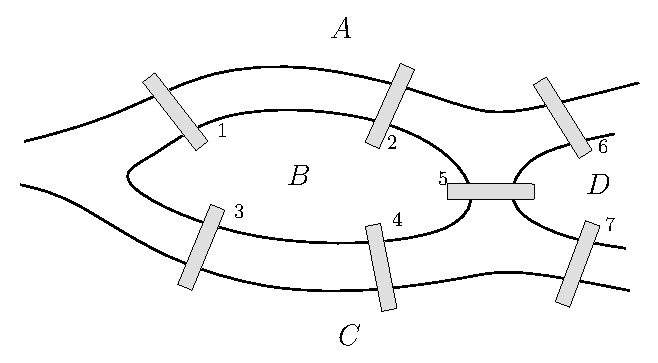
\includegraphics[height=150pt]{konigsberg}
\caption{Diagrama de la ciudad de K\"onigsberg.}
\label{fig:konigsberg}
\end{figure}

Los habitantes de K\"onigsberg se preguntaban si existía alguna forma de salir de casa, recorrer la ciudad pasando por todos los puentes una vez por cada uno, y regresar a casa.
En la figura~\ref{fig:graph1} se ha hecho una representación simplificada de la ciudad.
Cada punto representa una de las regiones, y cada trazo a un puente.
El problema puede reducirse entonces al de dibujar la figura~\ref{fig:graph1} sin levantar el lápiz y sin repetir ningún trazo, partiendo desde uno de los puntos y volviendo al inicial.

\begin{figure}[h!]
\centering
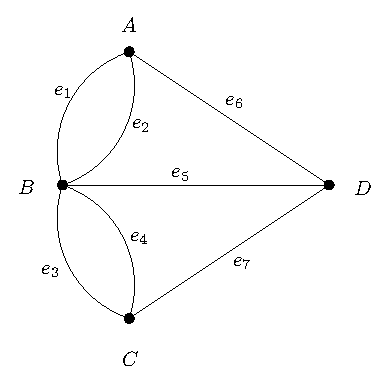
\includegraphics[height=150pt]{graph1}
\caption{Representación simplificada de la ciudad de K\"onigsberg.}
\label{fig:graph1}
\end{figure}

Con esta reformulación no es difícil argumentar que la respuesta al problema de los puentes es no.
Lo primero es notar que para dibujar la figura~\ref{fig:graph1} debemos para cada punto que no es el incial, ``entrar'' por un trazo y ``salir'' por otro trazo (distinto).
Si notamos en la figura el punto $D$ por ejemplo, tiene tres trazos ``incidiendo'' en él, por lo que después de que se pase por $D$ una vez (se ``entre y salga'' de $D$), la próxima vez que se llegue a $D$ no se podrá salir.
Lo mismo pasa con los puntos $A$ y $C$.
El punto $B$ es un poco diferente, dado que tiene $5$ trazos, se podrá ``entrar y salir'' dos veces, cuando se llegue por tercera vez a $B$ ya no se podrá salir.
El problema entonces surge porque los puntos tienen una cantidad impar de trazos.
Dado que el problema exige que el punto inicial sea igual al punto final, se puede concluir, por la misma razón, que tampoco es posible partir de ninguno de estos puntos ya que el trazo por el que se sale inicialmente de un punto debe ser distinto al con el que se llega finalmente.

El problema entonces tiene que ver con la paridad de los trazos de cada punto.
Basta con que uno de los puntos tenga una cantidad impar de trazos para que la figura no se pueda dibujar siguiendo las reglas pedidas.
Finalmente es imposible recorrer la ciudad completa de K\"onigsberg pasando por todos los punetes y volver a casa.
El primero que dio esta respuesta fue el matemático suizo L. Euler(1707--1783) en el año 1735.
\end{ejemplo}

\begin{ejemplo}
El ejemplo anterior era un poco radical porque todos sus puntos tenían una cantidad impar de trazos.
La figura~\ref{fig:graph2} tampoco se puede dibujar sin repetir trazos y volviendo al punto de partida.

\begin{figure}[h!]
\centering
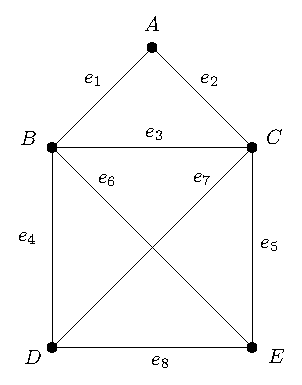
\includegraphics[height=150pt]{graph2}
\caption{Figura que tampoco se puede dibujar cumpliendo las reglas.}
\label{fig:graph2}
\end{figure}

La razón es la misma que antes, existen puntos con cantidad impar de trazos, en este caso los puntos $D$ y $E$ tienen ambos tres trazos.
Basta con que uno de los puntos de la figura tenga una cantidad impar de trazos para que esta no se pueda dibujar siguiendo las restricciones.
>Qué pasa si una figura tiene todos sus puntos con una cantidad par de trazos?
En este caso nuestra argumentación inicial no sería aplicable si quisiéramos mostrar que no se puede dibujar.
El resultado interesante que veremos más adelante, no dirá que para que una figura se pueda dibujar siguiendo las restricciones, simplemente basta con que todos sus puntos tengan una cantidad par de trazos.
De allí se concluirá que una figura se puede dibujar sin repetir trazos y volviendo al punto de partida, si y sólo si cada punto tiene una cantidad par de trazos.
\end{ejemplo}

Los anteriores ejemplo motivan nuestra definición de grafo.

\begin{definicion}
Un {\bf grafo} $G$ está compuesto por un conjunto de {\bf vértices} que llamaremos $V(G)$, un conjunto de {\bf aristas} que llamaremos $E(G)$, y una relación que a cada arista $e\in E(G)$ le asigna un par de vértices no necesariamente distintos de $V(G)$.

Para representar un grafo se usan puntos para dibujar vértices y trazos para dibujar aristas, cada arista se dibuja como un trazo entre los vértices con los que se encuentra relacionada.
\end{definicion}

\begin{ejemplo}
En ejemplo de la figura~\ref{fig:graph1} el conjunto de vértices es $\{A,B,C,D\}$ y el conjunto de aristas es $\{e_1,e_2,e_3,e_4,e_5,e_6,e_7\}$.
La asignación entre aristas y vértices se puede obtener de la figura, por ejemplo, la arista $e_5$ está relacionada con los vértices $B$ y $D$.

En ejemplo de la figura~\ref{fig:graph2} el conjunto de vértices es $\{A,B,C,D,E\}$ y el conjunto de aristas es $\{e_1,e_2,e_3,e_4,$ $e_5,e_6,e_7,e_8\}$.
La asignación entre aristas y vértices se puede obtener de la figura, por ejemplo, la arista $e_5$ está relacionada con los vértices $C$ y $E$.

Una diferencia importante entre los grafos de las figuras~\ref{fig:graph1} y~\ref{fig:graph2}, es que en el segundo, cada arista está relacionada con un par de vértices distintos.
Nuestra definición de grafo también permite por ejemplo que una arista esté relacionada con un par de vértices iguales.
En la figura~\ref{fig:graph3} se muestra un grafo con aristas de este tipo.
\begin{figure}[h!]
\centering
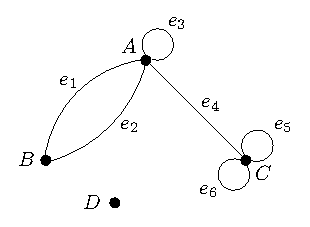
\includegraphics{graph3}
\caption{Grafo con rulos y aristas paralelas.}
\label{fig:graph3}
\end{figure}
En este grafo el conjunto de vértices es $\{A,B,C,D\}$ y el conjunto de aristas es $\{e_1,e_2,e_3,e_4,e_5,e_6\}$. 
La arista $e_6$ por ejemplo está relacionada con el vértice $C$ (o con el par de vértices $C$ y $C$).
Otra cosa interesante de este grafo es que ninguna arista está relacionada con el vértice $D$, esto para nada escapa de nuestra definición. 
\end{ejemplo}

\begin{definicion}
Un {\bf rulo} en un grafo, es una arista que está relacionada con sólo un vértice.
Dos aristas son {\bf paralelas} si sus pares de vértices relacionados son iguales.

Un grafo de dice {\bf simple} si no tiene rulos ni aristas paralelas.
El grafo de la figura~\ref{fig:graph2} es simple, mientras que los de las figuras~\ref{fig:graph1} y~\ref{fig:graph3} no lo son.

Una arista en un grafo simple puede verse como un par no ordenado de vértices.
Si la arista $e$ está relacionada con los vértices $u$ y $v$, escribiremos $e=uv$ o $e=vu$.
Así podremos decir que un grafo simple es un par $G=(V(G),E(G))$ donde los elementos de $E(G)$ son pares no ordenados de elementos de $V(G)$. 
En el grafo de la figura~\ref{fig:graph2}, podemos decir por ejemplo que $e_4=BD$ y que $e_7=CD$, luego el grafo es $G=(V(G),E(G))$ con $V(G)=\{A,B,C,D,E\}$ y $E(G)=\{AB,AC,BC,BD,CE,BE,CD,DE\}$.
En un grafo simple entonces no es necesario que las aristas tengan nombre, basta identificar al par de vértices que relacionan.
Cuando en un grafo simple $G$ exista una arista $uv\in E(G)$ diremos que $u$ y $v$ son {\bf vecinos} o vértices {\bf adyacentes}, así por ejemplo en el grafo de la figura~\ref{fig:graph2}, $A$ y $B$ son vértices vecinos, al igual que $D$ y $E$.
%
%Dado un grafo $G$, y un vertice cualquiera $v\in V(G)$, se define el {\bf grado} del vértice $v$ como la cantidad de aristas de $G$ que están relacionadas con $v$, cuando el grafo es simple, el grado de $v$ será simplemente la cantidad de vecinos de $v$.
%El grado de $v$ en $G$ lo denotamos por $\delta_G(v)$.
%Cuando el grafo al cual nos refiramos quede claro en el contexto, simplemente escribiremos $\delta(v)$ para referirnos al grado de $v$.

Nosotros estudiaremos principalmente grafos simples.
A menos que se explicite otra cosa, cuando nos refiramos a un grafo nos estaremos refiriendo a un grafo simple con un conjunto no vacío finito de vértices.
\end{definicion}

\subsection{Isomorfismos y Clases de Grafos}

>Cuando dos grafos son estructuralmente equivalentes?
Por ejemplo, >cuál es la diferencia entre los dos grafos de la figura~\ref{fig:compare-graph}?
\begin{figure}[t!]
\centering
\begin{tabular}{cc}
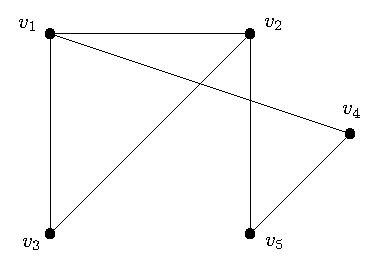
\includegraphics{graph5}\hspace*{3em} & \hspace*{3em}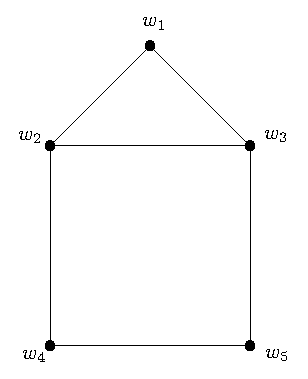
\includegraphics{graph4} \\
$G_1$ \hspace*{3em} & \hspace*{3em} $G_2$
\end{tabular}
\caption{>Cuál es la diferencia entre $G_1$ y $G_2$?}
\label{fig:compare-graph}
\end{figure}
Ciertamente los dibujos se ven distintos, sin embargo comparten algunas cosas como que ambos tienen la misma cantidad de vértices y la misma cantidad de aristas.
>Pero será que se ven distintos simplemente por la forma en que lo dibujamos?
>Podremos dibujarlos de manera que se ``vean'' iguales?
La respuesta es sí.
En la figura~\ref{fig:transform} se muestra como se pueden ``mover'' los vértices de $G_1$ de manera que se ``vea'' igual a $G_2$.
\begin{figure}[t!]
\centering
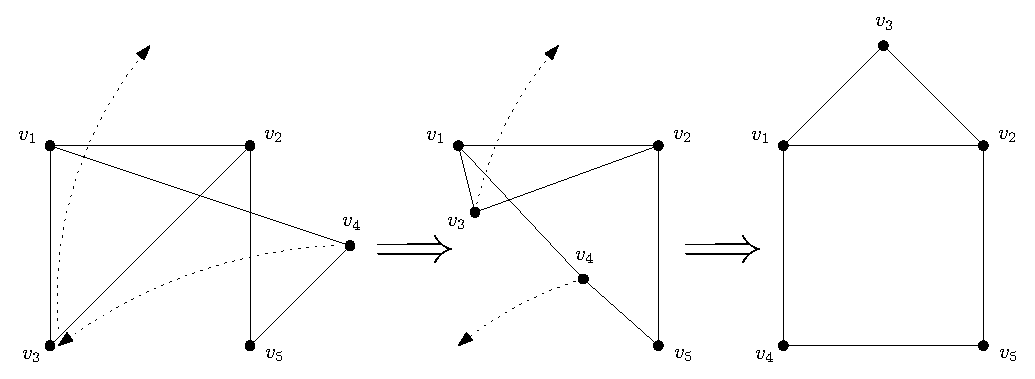
\includegraphics{graph8}\\
\caption{Transformación de $G_1$.}
\label{fig:transform}
\end{figure}
Lo que estamos haciendo es simplemente ``llevando'' $v_3$ a la posición que ocupa $w_1$ y $v_4$ a la posición que ocupa $w_4$.
Si ahora hacemos un ``renombre'' de los vértices de $G_1$ siguiendo la siguiente regla:
\[
\begin{array}{ccc}
v_1 & \rightarrow & w_2 \\
v_2 & \rightarrow & w_3 \\
v_3 & \rightarrow & w_1 \\
v_4 & \rightarrow & w_4 \\
v_5 & \rightarrow & w_5
\end{array}
\]
obtenemos exactamente a $G_2$.
Esto motiva nuestra definición de equivalencia entre grafos que llamaremos {\bf isomorfismo}.

\begin{definicion}
Dos grafos $G_1$ y $G_2$ se dicen {\bf isomorfos} si existe una función biyectiva $f$ desde $V(G_1)$ a $V(G_2)$, $f:V(G_1)\rightarrow V(G_2)$, tal que si $uv\in E(G_1)$ entonces $f(u)f(v)\in E(G_2)$, o sea, si hay una arista entre el par de vértices $u$ y $v$ en $G_1$, entonces hay una arista entre sus imágenes $f(u)$ y $f(v)$ en $G_2$.
Cuando se cumplan estas condiciones, diremos que $f$ es un {\bf isomorfismo} entre $G_1$ y $G_2$.
Escribiremos $G_1\cong G_2$ cuando $G_1$ y $G_2$ sean isomorfos.
No es difícil notar que $\cong$ es una relación de equivalencia entre grafos.
\end{definicion}

\begin{ejemplo}
Los grafos $G_1$ y $G_2$ de la figura~\ref{fig:compare-graph} son isomorfos.
Para demostrarlo basta encontrar una función $f$ biyectiva que cumpla con ser un isomorfismo entre $G_1$ y $G_2$.
La función $f$ es la que ya detallamos:
\[
\begin{array}{ccc}
& f \\
v_1 & \rightarrow & f(v_1)=w_2 \\
v_2 & \rightarrow & f(v_2)=w_3 \\
v_3 & \rightarrow & f(v_3)=w_1 \\
v_4 & \rightarrow & f(v_4)=w_4 \\
v_5 & \rightarrow & f(v_5)=w_5
\end{array}
\]
Primero $f$ es claramente biyectiva.
Ahora debemos comprobar que efectivamente es un isomorfismo, para esto debemos chequear que para cada par de vértices que forman una arista en $G_1$, sus imágenes también forman una arista en $G_2$.
\[
\begin{array}{lclcccccc}
v_1v_2\in E(G_1), & & f(v_1)f(v_2)=w_2w_3 \in E(G_2) \\
v_1v_3\in E(G_1), & & f(v_1)f(v_3)=w_2w_1 \in E(G_2) \\
v_1v_4\in E(G_1), & & f(v_1)f(v_4)=w_2w_4 \in E(G_2) \\
v_2v_3\in E(G_1), & & f(v_2)f(v_3)=w_3w_1 \in E(G_2) \\
v_2v_5\in E(G_1), & & f(v_2)f(v_5)=w_3w_5 \in E(G_2) \\
v_5v_4\in E(G_1), & & f(v_5)f(v_4)=w_5w_4 \in E(G_2) \\
\end{array}
\]
Finalmente $f$ es un isomorfismo de donde concluimos que $G_1\cong G_2$.
\end{ejemplo}
Más adelante veremos técnicas que nos ayudarán a determinar cuándo dos grafos no son isomorfos, por ahora el alumno puede notar que por ejemplo, una condición necesaria (pero no suficiente) para que dos grafos sean isomorfos es que tengan la misma cantidad de vértices y la misma cantidad de aristas.

Otro punto interesante del isomorfismo de grafos y que tiene que ver con computación, es que hasta el día de hoy, nadie ha podido encontrar un algoritmo ``eficiente'' para determinar si dos grafos cualquiera son o no isomorfos.
Volveremos a este punto cuando en el siguiente capítulo definamos la noción de eficiencia de un algoritmo.

La relación $\cong$ es una relación de equivalencia, como tal define clases de equivalencias sobre el conjunto de los grafos.
Estudiaremos algunas de estas clases de equivalencia y les daremos nombre.

\subsection{Algunas Clases de Grafos}

Comenzaremos con un par de definiciones.
\begin{definicion}
Un {\bf camino} es un grafo simple cuyos vértices pueden \emph{ordenarse en una linea} de manera tal que dos vértices son adyacentes si y sólo si son consecutivos en la lista.
Un {\bf ciclo} es un grafo simple cuyos vértices pueden disponerse \emph{en círculo} de manera que dos vértices son adyacentes si y sólo si aparecen en posiciones consecutivas en un círculo.
Un ejemplo de camino y ciclo se muestra en la figura~\ref{fig:graph9}
\begin{figure}[h!]
\centering
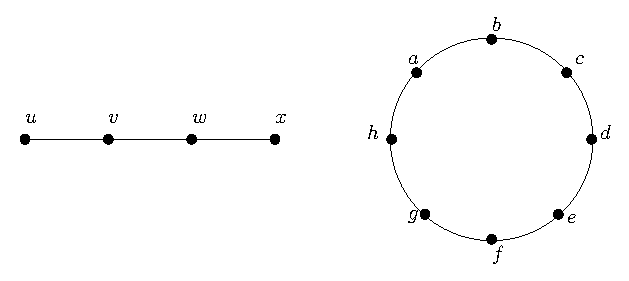
\includegraphics[height=85pt]{graph9}\\
\caption{Un camino (izquierda) y un ciclo (derecha).}
\label{fig:graph9}
\end{figure}
\end{definicion}

\begin{definicion}
La \emph{clase de equivalencia} de todos los caminos con $n$ vértices la llamaremos $P_n$. 
La \emph{clase de equivalencia} de todos los ciclos con $n$ vértices la llamaremos $C_n$.
En general en vez de hablar de \emph{clase de equivalencia} de grafos, simplemente hablaremos de un grafo particular representante de esta clase, tal que al dibujarlo no nombraremos sus vértices.
Siguiendo esta norma, en la figura~\ref{fig:paths} aparecen $P_4$ y $P_6$.
\begin{figure}[h!]
\centering
\begin{tabular}{cc}
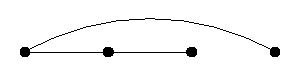
\includegraphics{p4}\hspace*{3em} &  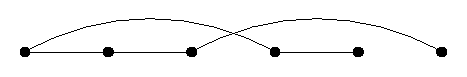
\includegraphics{p6} \\
$P_4$\hspace*{3em} & $P_6$
\end{tabular}
\caption{Clases de equivalencia para el camino de 4 y 6 vértices.}
\label{fig:paths}
\end{figure}
En ella $P_4$ y $P_6$ se han dibujado a propósito en una disposición no lineal, para enfatizar que lo que importa es su estructura más que el dibujo.
En la figura~\ref{fig:cycle} aparece $C_6$.
\begin{figure}[h!]
\centering
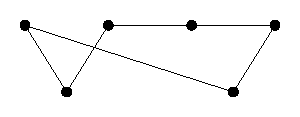
\includegraphics{c6}\\
$C_6$
\caption{Ejemplo del ciclo con 6 vértices.}
\label{fig:cycle}
\end{figure}
\end{definicion}

Otra clase de grafos importantes es el grafo completo.

\begin{definicion}
Un {\bf grafo completo} es un grafo simple en el que todos los pares de vértices son adyacentes.
Al grafo completo de $n$ vértices le llamaremos $K_n$.
En la figura~\ref{fig:cliques} se pueden ver a los grafos $K_n$ para $n=1,2,3,4,5$.
\begin{figure}[h!]
\centering
\begin{tabular}{ccccc}
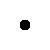
\includegraphics{k1}&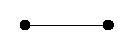
\includegraphics{k2}&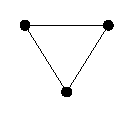
\includegraphics{k3}&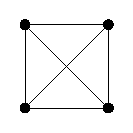
\includegraphics{k4}&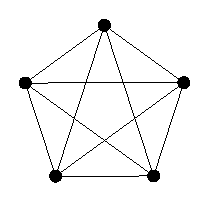
\includegraphics{k5}\\
$K_1$ & $K_2$ & $K_3$ & $K_4$ & $K_5$
\end{tabular}
\caption{Grafos completos.}
\label{fig:cliques}
\end{figure}
\end{definicion}

\begin{definicion}
Un grafo $G$ se dice {\bf bipartito} si $V(G)$ se puede agrupar en dos conjuntos disjuntos $V_1$ y $V_2$, $V_1\cap V_2=\emptyset$, $V_1\cup V_2=V(G)$, tal que toda arista en $E(G)$ une a un vértice de $V_1$ con uno de $V_2$.
Esto quiere decir que dos vértices de $V_1$ no pueden ser adyacentes, lo mismo con $V_2$.
\end{definicion}
\begin{figure}[h!]
\centering
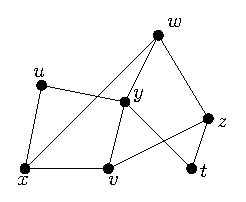
\includegraphics{graph10}\\
$G$
\caption{Ejemplo de un grafo bipartito}
\label{fig:graph10}
\end{figure}

\begin{ejemplo}
El grafo $G$ de la figura~\ref{fig:graph10} es un grafo bipartito.
El conjunto de vértices de $G$ es $V(G)=\{t,u,v,w,x,y,z\}$, que se puede separar en los conjuntos $V_1=\{t,u,v,w\}$ y $V_2=\{x,y,z\}$ tal que toda arista en $E(G)$ une a un vértice de $V_1$ con uno de $V_2$.
En general, cuando dibujemos un grafo bipartito haremos una clara separación entre las particiones de los vértices ($V_1$ y $V_2$) dibujando los vértices de una de las particiones ``arriba'' de los vértices de la otra partición.
En la figura~\ref{fig:graph11} se ha seguido esta norma para dibujar nuevamente a $G$.
\begin{figure}[h!]
\centering
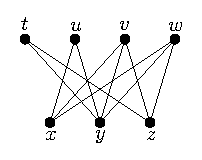
\includegraphics{graph11}\\
$G$
\caption{El mismo grafo bipartito haciendo una clara diferencia en las particiones.}
\label{fig:graph11}
\end{figure}  
\end{ejemplo}

\begin{ejemplo}
Los grafos bipartitos generalmente se usan para modelar problemas de \emph{asignación} de recursos o tareas.
Podemos suponer que hay vértices de un grafo representando personas y tareas, y que un vértice $p$ correspondiente a una persona es adyacente a un vértice $t$ correspondiente a una tarea si es que la persona $p$ está capacitada para realizar la tarea $t$.
Un grafo de estas características siempre será bipartito.
Un ejemplo se ve en la figura~\ref{fig:job-ass}.
Una pregunta que se puede hacer sobre este tipo de grafos es si existe alguna forma de asignar las tareas de manera tal que toda puedan ser realizadas simultáneamente.
\begin{figure}[h!]
\centering
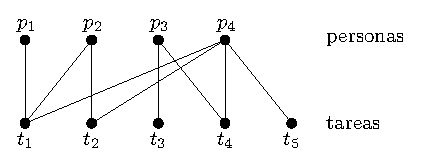
\includegraphics{graph12}
\caption{Un grafo para modelar un problema de asignación de tareas.}
\label{fig:job-ass}
\end{figure} 
En el grafo de ejemplo esto no es posible (>por qué?).
Más adelante en el curso veremos algunos resultado que nos permitirán establecer cuándo y cuándo no se puede hacer una asignación en grafos de este tipo.
\end{ejemplo}

\begin{definicion}
Un grafo {\bf bipartito completo} es un grafo bipartito en que cada uno de los vértices de una de las particiones es adyacente con cada uno de los vértices de la otra partición.
Cuando las particiones tengan $n$ y $m$ vértices, llamaremos $K_{n,m}$ al grafo bipartito completo.
En la figura~\ref{fig:k2-3} se muestra un diagrama para $K_{2,3}$.
\begin{figure}[h!]
\centering
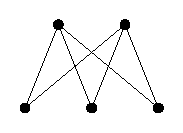
\includegraphics{k2-3}\\
$K_{2,3}$
\caption{El grafo bipartito completo cuyas particiones tienen tamaño 2 y 3.}
\label{fig:k2-3}
\end{figure}
\end{definicion}

En los siguientes ejemplos estudiaremos dos grafos muy importantes en la teoría, el hipercubo y el grafo de Petersen.

\begin{ejemplo}[El Hipercubo.]
Generalmente se utilizan grafos para representar la \emph{topología} de un conjunto de computadores (o procesadores) conectados por red.
Esta red de computadores podrá ejecutar algoritmos \emph{en paralelo} y la eficiencia de estos algoritmos muchas veces tiene que ver con la forma en la que los computadores se encuentran conectados para poder interactuar.
Un tipo de red muy eficiente y para el cual existen una cantidad considerable de algoritmos paralelos, es la llamada red de {\bf hipercubo}.

Un hipercubo $n$--dimensional, que llamaremos $H_n$, es un grafo simple en el que sus vértices han sido numerados en binario desde el $0$ al $2^n-1$, o sea cada vértice tiene un nombre compuesto por $n$ bits.
Una arista conecta a un par de vértices del hipercubo si estos difieren exactamente en un bit.
Así por ejemplo, el hipercubo de 3 dimensiones, $H_3$, tiene $8$ vértices, $V(H_3)=\{000,001,010,011,100,101,110,111\}$ y es tal que hay una arista entre $010$ y $110$, entre $111$ y $011$, etc.
Un diagrama de $H_3$ se puede ver en la figura~\ref{fig:h3}.
\begin{figure}[h!]
\centering
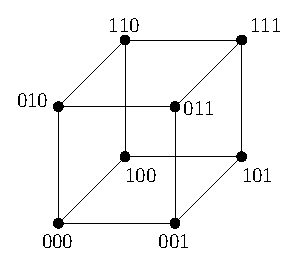
\includegraphics{h3}\\
$H_3$
\caption{El hipercubo de 3 dimensiones.}
\label{fig:h3}
\end{figure}

Una primera observación es que $H_n$ es un grafo bipartito para todo $n$.
De hecho si tomamos $V_1$ como todos los vértices de $V(H_n)$ que tienen una cantidad par de $1's$ y $V_2$ como todos los vértices que tienen una cantidad impar de $1's$ es claro que toda arista en $E(H_n)$ unirá siempre a un vértice de $V_1$ con uno de $V_2$.

Otra observación importante es que un hipercubo $n$--dimensional puede ser creado en forma recursiva a partir de dos hipercubos de dimensión $n-1$.
Supongamos que tenemos dos hipercubos de dimensión $n-1$, $H'$ y $H''$, cada uno de ellos tiene $2^{n-1}$ vértices numerados desde el $0$ al $2^{n-1}-1$.
Podemos crear un hipercubo $n$--dimensional a partir de $H'$ y $H''$ añadiendo una arista entre cada par de vértices de $H'$ y $H''$ que tienen el mismo número binario asignado y posteriormente cambiar los nombres de los vértices de $V(H')$ agregándoles un $0$ al inicio, y los de $V(H'')$ agregándoles un $1$ al inicio.
El caso base de esta construcción es el hipercubo $H_1$ que tiene vértices $0$ y $1$, y una arsita uniéndolos.
La figura~\ref{fig:h4} muestra la construcción de $H_4$ a partir de dos instancias de $H_3$.
\begin{figure}[h!]
\centering
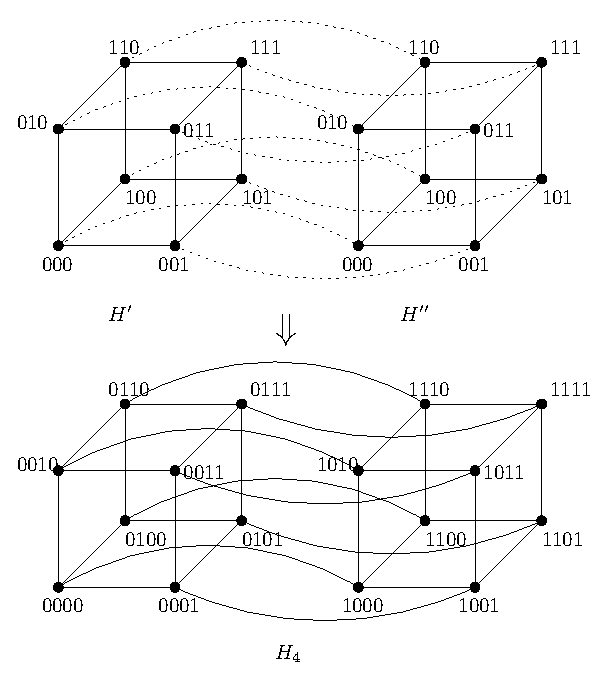
\includegraphics{h4}
\caption{Construcción de $H_4$ a partir de dos copias de $H_3$.}
\label{fig:h4}
\end{figure}

Esta última forma de construcción nos da un manera de establecer algunas propiedades de conteo recursivas acerca de $H_n$.
Por ejemplo podemos contar cuántas aristas tiene $H_n$ a partir de establecer una fórmula recursiva para $|E(H_n)|$ en función de $|E(H_{n-1})|$, usando la construcción no es difícil obtener que:
\[
\begin{array}{rcl}
|E(H_n)|&=&2^{n-1}+2|E(H_{n-1})| \\
|E(H_1)|&=&1
\end{array}
\]
Como ejercicio el alumno podría obtener una fórmula explicita para $|E(H_n)|$ usando la recurrencia anterior.
\end{ejemplo}

\begin{ejemplo}[El Grafo de Petersen.]
El grafo de Petersen, que llamaremos $Pet$ es un grafo simple cuyos vértices son los subconjuntos de dos elementos de $\{0,1,2,3,4\}$, por ejemplo $\{0,1\}$, $\{2,4\}$ y $\{1,3\}$ son vértices en el grafo de Petersen.
Dos vértices $A$ y $B$ del grafo de Petersen están unidos por una arista si ocurre que $A\cap B=\emptyset$.
Formalmente podemos definir entonces al grafo de Petersen, como un grafo $G=(V(G),E(G))$ tal que:
\[
\begin{array}{l}
V(G)=\{A\;|\;A\subseteq \{0,1,2,3,4\}\,\wedge\, |A|=2\} \\
E(G)=\{AB\;|\;A,B\in V(G)\,\wedge\, A\cap B=\emptyset\}
\end{array}
\]
En la figura~\ref{fig:petersen} se muestra tres formas distintas de dibujar al grafo de Petersen.
Para mostrar que ellos son efectivamente isomorfos al grafo de Petersen, basta con nombrar sus vértices como subconjuntos de tamaño 2 de $\{0,1,2,3,4\}$ y verificar que sus aristas unen a los vértices correspondientes.
\begin{figure}[h!]
\centering
\begin{tabular}{ccc}
  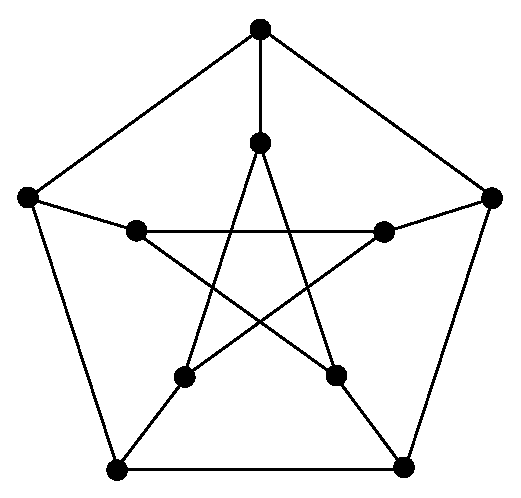
\includegraphics[height=100pt]{pet2.eps} \hspace*{1cm}&
  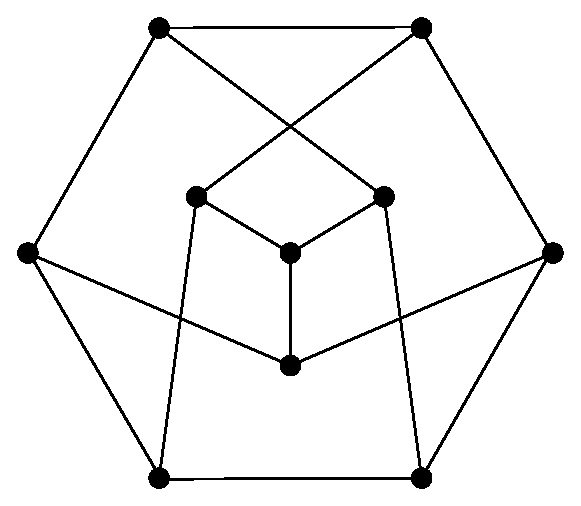
\includegraphics[height=100pt]{pet3.eps} & \hspace*{1cm}
  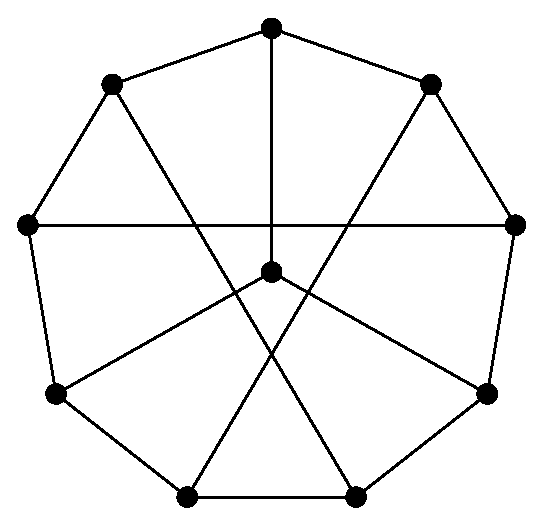
\includegraphics[height=100pt]{pet1.eps} 
  \end{tabular}
\caption{Tres formas de dibujar el grafo de Petersen.}
\label{fig:petersen}
\end{figure}

Se pueden establecer varias propiedades interesantes del grafo de Petersen, sin necesidad de analizar sus dibujos, usando sólo su definición abstracta.
Primero, el grafo tiene exactamente 10 vértices, que es la cantidad de subconjuntos de dos elementos que se pueden hacer sobre el conjunto $\{0,1,2,3,4\}$.
Otra propiedad tiene que ver con la cantidad de vecinos que cada vértice tiene en el grafo de Petersen.
Sea $A$ un vértice cualquiera, sabemos que $|A|=2$ y por lo tanto el conjunto $A'=\{0,1,2,3,4\}-A$ es tal que $|A'|=3$.
Cada vértice de $A$ se obtendrá a partir de un subconjunto de tamaño 2 de $A'$, como hay exactamente $3$ de tales subconjuntos, $A$ tiene $3$ vecinos.
Otra propiedad interesante es la siguiente, dados dos vértices no adyacentes en el grafo, ellos tienen exactamente un vecino en común.
Esto se puede demostrar con el siguiente argumento, dados dos vértices distintos $A$ y $B$, estos no son vecinos si ocurre que $A\cap B\not=\emptyset$, esto quiere decir que el conjunto $A\cup B$ tiene exactamente $3$ elementos.
Un vértice que sea simultáneamente vecino de $A$ y $B$ debe ser entonces un subconjunto de dos elementos del conjunto $\{0,1,2,3,4\}-(A\cup B)$, y dado que este conjunto tiene exactamente $2$ elementos, él representa al único vecino común entre $A$ y $B$.
\end{ejemplo}

%Terminamos esta subsección con un par de definiciones importantes en la teoría de grafos.

\begin{definicion}
Dado un grafo $G=(V(G),E(G))$, diremos que $H=(V(H),E(H))$ es un {\bf subgrafo} de $G$ si $V(H)\subseteq V(G)$, $E(H)\subseteq E(G)$, y en $E(H)$ aparecen sólo aristas que unen a vértices de $V(H)$.
Cuando $H$ sea subgrafo de $G$, escribiremos $H\subseteq G$.

Un {\bf clique} en un grafo $G$ es un conjunto de vértices $K\subseteq V(G)$ en que para cada par de vértices $u,v\in K$, la arista $uv\in E(G)$.
Un {\bf conjunto independiente} en un grafo $G$ es un conjunto de vértices $K\subseteq V(G)$ tal que para cada par de vértices $u,v\in K$, la arista $uv\notin E(G)$.
El tamaño de un clique o de un conjunto independiente es la cantidad de vértices que lo componen.
\end{definicion}

\begin{ejemplo}
Para el grafo completo $K_n$, se cumple que $\forall i\leq n$, $K_i\subseteq K_n$.
También se cumple que cualquier subconjunto de $V(K_n)$ es un clique en $K_n$.
Los únicos conjuntos independientes en $K_n$ son los conjuntos compuestos por un único vértice de $V(K_n)$.

Para el grafo bipartito completo $K_{n,m}$ con particiones $V_1$ y $V_2$, tanto $V_1$ como $V_2$ son conjuntos independientes.
El clique más grande que se puede encontrar en $K_{n,m}$ está compuesto por dos vértices >por qué?.
Podemos decir también que $C_3$ nunca es subgrafo de $K_{n,m}$,
>puede ocurrir que $C_4\subseteq K_{n,m}$?
>puede ocurrir que $C_5\subseteq K_{n,m}$?
\end{ejemplo}

\begin{definicion}
Dado un grafo $G=(V(G),E(G))$ definimos el {\bf complemento} de $G$ como el grafo $\overline{G}=(V(G),E(\overline{G}))$, en donde el conjunto de arista cumple con $uv\in E(\overline G)\Leftrightarrow uv\notin E(G)$,
o sea $\overline G$ se obtiene a partir de los vértices de $G$ agregando una arista entre cada par de vértices no vecinos en $G$.
Un grafo $G$ se dice {\bf autocomplementario} si ocurre que $G\cong\overline G$.
\end{definicion}

El siguiente teorema nos da una relación entre cliques, conjuntos independientes y el grafo complemento.

\begin{teorema}
\label{teo:clique-indep}
Dado un grafo $G=(V(G),E(G))$ y un subconjunto $V\subseteq V(G)$, entonces $V$ es un clique en $G$ si y sólo si $V$ es un conjunto independiente en $V(\overline G)$.

\begin{demostracion}
Supongamos que $V\subseteq V(G)$ es un clique en $G$, esto quiere decir que para todo $u,v\in V$ ocurre que $uv\in E(G)$.
Por la definición de $\overline G$, sabemos que para todo $u,v\in V$ ocurre que $uv\notin E(\overline G)$ por lo tanto $V$ es un conjunto independiente en $\overline G$.
La implicación inversa se obtiene de manera similar.
\end{demostracion}
\end{teorema}

\begin{ejemplo}
En la figura~\ref{fig:complementos} se muestran tres grafos y sus grafos complemento.
En ella podemos ver que por ejemplo $P_4$ es autocomplementario, que $P_5$ no es autocomplementario, y que el complemento de $K_4$ es un grafo de $4$ vértices \emph{aislados}, ninguno es vecino de otro.
\begin{figure}[h!]
\centering
\begin{tabular}{cc}
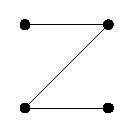
\includegraphics{p4-2}\hspace*{3em} &  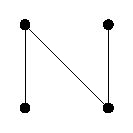
\includegraphics{p4-2c} \\
$P_4$\hspace*{3em} & $\overline{P_4}$ \\
& \\
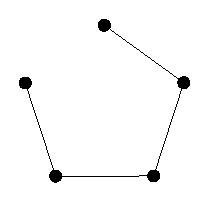
\includegraphics{p5}\hspace*{3em} &  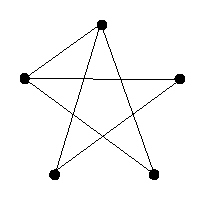
\includegraphics{p5c} \\
$P_5$\hspace*{3em} & $\overline{P_5}$ \\
& \\
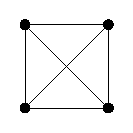
\includegraphics{k4}\hspace*{3em} &  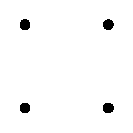
\includegraphics{k4c} \\
$K_4$\hspace*{3em} & $\overline{K_4}$
\end{tabular}
\caption{Algunos grafos y sus complementos}
\label{fig:complementos}
\end{figure}
\end{ejemplo}

\begin{ejemplo}
Dado un conjunto de 6 personas >es cierto que siempre ocurre que hay, o bien tres personas que se conocen mutuamente, o bien tres personas que se desconocen mutuamente?
La respuesta a esta pregunta es SI, y lo justificaremos  modelando el problema con grafos.

Podemos usar un grafo $G$ con 6 vértices $\{p_1,p_2,p_3,p_4,p_5,p_6\}$, cada uno representando a una persona, y agregar la arista $p_ip_j$ si las personas $p_i$ y $p_j$ se conocen.
Queremos demostrar entonces que en cualquier grafo $G$ de 6 vértices ocurre que este o contiene un clique de tamaño 3, o contiene un conjunto independiente de tamaño 3.
Similarmente y usando el teorema~\ref{teo:clique-indep} podemos decir que el problema es equivalente a demostrar que para cualquier grafo de 6 vértices ocurre que, o $G$ tiene un clique de tamaño 3, o $\overline G$ tiene un clique de tamaño 3.
En la figura~\ref{fig:clique-indep} se muestra un posible grafo de $6$ vértices junto a su complemento.
\begin{figure}[h!]
\centering
\begin{tabular}{cc}
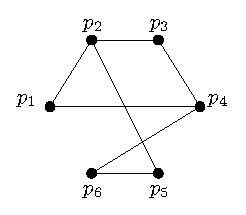
\includegraphics{graph13}\hspace*{3em} &  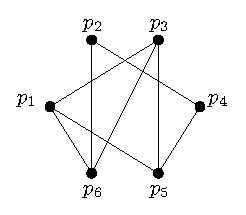
\includegraphics{graph14} \\
$G$\hspace*{3em} & $\overline G$
\end{tabular}
\caption{Conocidos mutuos y desconocidos mutuos}
\label{fig:clique-indep}
\end{figure}
En el podemos ver que $G$ no tiene un clique de tamaño 3, pero que $\overline G$ si lo tiene, por lo tanto hay tres personas que se desconocen mutuamente (de hecho hay dos de estos grupos, $\{p_1,p_3,p_6\}$ y $\{p_1,p_3,p_5\}$).

Lo que sigue de la demostración la haremos por contradicción suponiendo que ni $G$ ni $\overline G$ tienen un clique de tamaño 3.
La primera observación que haremos es la siguiente:
si miramos una persona en particular, esta o se conoce con al menos tres personas, o se desconoce con al menos tres personas, esto es equivalente a decir que dado un vértice $v$ cualquiera ocurre que, o la cantidad de vecinos de $v$ en $G$ es mayor o igual a 3, o la cantidad de vecinos de $v$ en $\overline G$ es mayor o igual a 3, esto es inmediato del hecho de que todas las aristas que faltan en $G$ aparecen en $\overline G$ (y vice versa).

Enfoquémonos en un vértice en particular $p_i$ y supongamos que su cantidad de vecinos es mayor o igual a 3 en $G$, entonces existen otros tres vértices distintos a $p_i$ y distintos entre sí, $p_j$, $p_k$ y $p_l$ que son vecinos de $p_i$.
Dado que estamos suponiendo que $G$ no tiene un clique de tamaño 3, entonces necesariamente en $G$ $p_j$ no es vecino de $p_k$, $p_j$ no es vecino de $p_l$, y $p_k$ no es vecino de $p_l$, lo que implica que en $\overline G$ los vértices $p_j$, $p_k$ y $p_l$ forman un clique de tamaño tres contradiciendo nuestra suposición de que $\overline G$ no tiene un clique de tamaño 3 (ver figura~\ref{fig:graph15})
Si por el contrario resulta que el vértice particular $p_i$ en el que nos estamos enfocando tiene menos de tres vecinos en $G$, necesariamente este tiene una cantidad de vecinos mayor o igual a 3 en $\overline G$ y podemos usar exactamente el mismo argumento partiendo de $\overline G$ y contradiciendo la suposición de que $G$ no tiene un clique de tamaño 3.
\begin{figure}[h!]
\centering
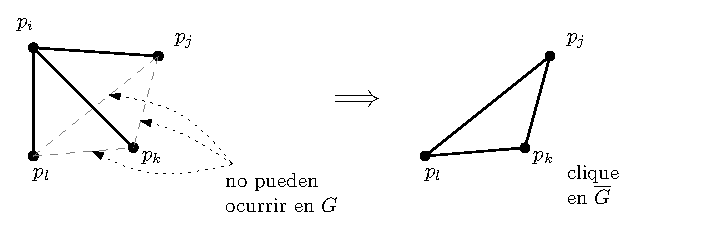
\includegraphics{graph15}
\caption{Conocidos y desconocidos mutuos.}
\label{fig:graph15}
\end{figure}
\end{ejemplo}

\subsection{Representación Matricial}

Podemos usar una matriz $M_G$ para representar cualquier grafo simple $G$ usando la matriz que representa a la relación \emph{ser vecino de} entre los vértices de $G$, $V(G)$.
Claramente la relación de ser vecino es simétrica por lo que se cumplirá que $M_G=(M_G)^T$, además, dado que $G$ es un grafo simple, la diagonal de $G$ tendrá sólo 0's.
A la matriz $M_G$ se le llama {\bf matriz de adyacencia} de $G$.
Si $G$ tiene $n$ nodos entonces $M_G$ será una matriz de $n\times n$.

\begin{ejemplo}
Para el grafo $G$ de la figura~\ref{fig:clique-indep} la matriz de adyacencia $M_G$ resulta
\[
M_G=
\begin{array}{cc}
& \hspace*{-1.5em}
\begin{array}{ccccccccccc}
p_1\hspace*{-0.5em}& p_2\hspace*{-0.5em} & p_3\hspace*{-0.5em} & p_4\hspace*{-0.5em} & p_5\hspace*{-0.5em} & p_6
\end{array}\\
\begin{array}{c}
p_1\\
p_2\\
p_3\\
p_4\\
p_5\\
p_6
\end{array}
& \hspace*{-1.5em}
\left[
\begin{array}{ccccccccc}
0&1&0&1&0&0 \\
1&0&1&0&1&0 \\
0&1&0&1&0&0 \\
1&0&1&0&0&1 \\
0&1&0&0&0&1 \\
0&0&0&1&1&0 \\
\end{array}
\right]
\end{array}
\]
en donde las filas se han organizado en el orden de los índices de los vértices.
Por su parte la matriz para el grafo $\overline G$ de la misma figura es
\[
M_{\overline G}=
\begin{array}{cc}
& \hspace*{-1.5em}
\begin{array}{ccccccccccc}
p_1\hspace*{-0.5em}& p_2\hspace*{-0.5em} & p_3\hspace*{-0.5em} & p_4\hspace*{-0.5em} & p_5\hspace*{-0.5em} & p_6
\end{array}\\
\begin{array}{c}
p_1\\
p_2\\
p_3\\
p_4\\
p_5\\
p_6
\end{array}
& \hspace*{-1.5em}
\left[
\begin{array}{ccccccccc}
0&0&1&0&1&1 \\
0&0&0&1&0&1 \\
1&0&0&0&1&1 \\
0&1&0&0&1&0 \\
1&0&1&1&0&0 \\
1&1&1&0&0&0 \\
\end{array}
\right]
\end{array}
\]
No es difícil justificar que si $M_G$ es la matriz de adyacencia para $G$, entonces la matriz de adyacencia para $\overline G$ se puede obtener de $M_G$ intercambiando todos los $0$'s por $1$'s excepto en la diagonal.
\end{ejemplo}

La matriz de adyacencia es una forma en que un grafo se le puede entregar a un computador para realizar cierta tarea sobre él.
>Qué pasa cuando $G$ no es un grafo simple?
Supongamos que $G$ es un grafo no necesariamente simple, pero sin rulos, entonces podríamos usar una matriz de adyacencia $M_G$ \emph{extendida} con no solo $0$'s y $1$'s, en que la posición $[M_G]_{(i,j)}=n$ si hay $n$ aristas incidiendo en los vértices que representados por $i$ y $j$.

\begin{ejemplo}
Para el gafo de la figura~\ref{fig:graph16} la matriz de adyacencia \emph{extendida} resulta
\[
\begin{array}{cc}
& \hspace*{-1.2em}
\begin{array}{ccccc}
A&B&C&D\\
\end{array}\\
\begin{array}{c}
A\\
B\\
C\\
D
\end{array}
& \hspace*{-1.2em}
\left[
\begin{array}{ccccc}
0&2&1&1\\
2&0&0&0\\
1&0&0&2\\
1&0&2&0
\end{array}
\right]
\end{array}
\]
en ella las filas se han organizado en el orden alfabético de los vértices.
\end{ejemplo}

Otra forma de representar un grafo matricialmente es usando lo que se llama la {\bf matriz de incidencia}.
En ella las filas se etiquetan con los vértices de $G$ y las columnas con las aristas de $G$.
Si suponemos que $G$ es un grafo no necesariamente simple, pero sin rulos, para cada columna representante de una arista, habrán dos $1$'s uno por cada vértice extremo de la arista.
Si $G$ tiene $n$ vértices y $m$ aristas, entonces su matriz de incidencia será una matriz de $n\times m$.

\begin{ejemplo}
Para el grafo de la figura~\ref{fig:graph16} la matriz de incidencia asociada será
\begin{figure}
\centering
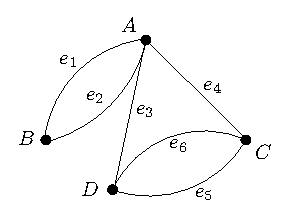
\includegraphics{graph16}
\caption{Un grafo sin rulos.}
\label{fig:graph16}
\end{figure}
\[
\begin{array}{cc}
& \hspace*{-1.2em}
\begin{array}{ccccccccccc}
e_1\hspace*{-0.5em}&e_2\hspace*{-0.5em}&e_3\hspace*{-0.5em}&e_4\hspace*{-0.5em}&e_5\hspace*{-0.5em}&e_6
\end{array}\\
\begin{array}{c}
A\\
B\\
C\\
D
\end{array}
& \hspace*{-1.2em}
\left[
\begin{array}{ccccccccccccc}
1&1&1&1&0&0\\
1&1&0&0&0&0\\
0&0&0&1&1&1\\
0&0&1&0&1&1
\end{array}
\right]
\end{array}
\]
\end{ejemplo}

Las matrices de adyacencia e incidencia de un grafo $G$ nos sirven para obtener propiedades del grafo y algunas otras propiedades interesantes de conteo. 
Por ejemplo, en un grafo simple si sumamos una fila de la matriz, el resultado es la cantidad de vecinos que tiene el vértice asociado a esa fila.
La siguiente definición tiene que ver con estas propiedades.

\begin{definicion}
El {\bf grado} de un vértice $v$ en un grafo $G$ sin rulos, es la cantidad de aristas de $E(G)$ que están asociadas a $v$.
Cuando $G$ sea un grafo simple el grado de $v$ coincidirá con la cantidad de vecinos.
Al grado del vértice $v$ en el grafo $G$ lo denotaremos por $\delta_G(v)$.
Cuando el grafo que estemos usando quede claro por el contexto, usaremos simplemente $\delta(v)$.
\end{definicion}

La primera implicación interesante para el grado de un vértice tiene que ver con las matrices de adyacencia e incidencia.
Sea $G$ un grafo sin rulos con $n$ vértices y $m$ aristas.
Si al vértice $v_i$ se asocia la fila $i$ de la matriz de adyacencia $M_G$ entonces se cumple que 
\[
\delta_G(v_i)=\sum_{j=1}^{n}[M_G]_{(i,j)}.
\]
Si al vértice $v_i$ se asocia la fila $i$ de la matriz de incidencia $A_G$ entonces se cumple que
\[
\delta_G(v_i)=\sum_{j=1}^{m}[A_G]_{(i,j)}.
\]

Otra propiedad que se puede obtener a partir de la matriz de incidencia tiene que ver con la relación entre los grados de los vértices y la cantidad de arista de un grafo.
Supongamos que tenemos un grafo $G$ sin rulos con $n$ vértices $v_1,v_2,\ldots,v_n$ y $m$ aristas $e_1,e_2,\ldots,e_m$.
Si tomamos la matriz de incidencia de $G$, $A_G$ y sumamos todos los $1$'s que aparecen en ella, esta suma resulta a partir de la doble sumatoria
\begin{equation}\label{eq:incidence-sum}
\sum_{i=1}^{n}\sum_{j=1}^{m}[A_G]_{(i,j)}
\end{equation}
y por el resultado anterior tenemos que
\begin{equation}\label{eq:sum-degree}
\sum_{i=1}^{n}\sum_{j=1}^{m}[A_G]_{(i,j)}=\sum_{i=1}^{n}\delta_G(v_i),
\end{equation}
lo único que hicimos fue reemplazar la sumatoria interna por el grado del vértice correspondiente a la fila que se está sumando.
Ahora si en la expresión~(\ref{eq:incidence-sum}) invertimos el orden de las sumatorias obtenemos
\[
\sum_{j=1}^{m}\sum_{i=1}^{n}[A_G]_{(i,j)}.
\]
Si miramos la nueva sumatoria interna $\sum_{i=1}^{n}[A_G]_{(i,j)}$ su resultado es siempre $2$ para cualquier $j$, esto porque én ella se están sumando los $1$'s que aparecen en una columna determinada de $A_G$, que sabemos que es $2$ porque hay un $1$ por cada vértice extremo de la arista correspondiente a esa columna, con lo que obtenemos
\begin{equation}\label{eq:two-edges}
\sum_{j=1}^{m}\sum_{i=1}^{n}[A_G]_{(i,j)}\sum_{j=1}^{m}2=2m.
\end{equation}
Dado que el orden en que se realizen las sumatorias no altera el resultado, a partir de~(\ref{eq:two-edges}) y~(\ref{eq:sum-degree}) obtenemos la igualdad
\[
\sum_{i=1}^{n}\delta_G(v_i)=2m,
\]
es decir, la suma total de los grados de los vértices es igual al doble de la cantidad de aristas.
Un elegante argumento de conteo del mismo resultado se puede ver en el siguiente diagrama:
\[
\begin{array}{cccc}
& 
\begin{array}{ccccccccccc}
e_1&e_2&e_3&\cdots&e_m
\end{array}
\\
\begin{array}{c}
v_1\\
v_2\\
\vdots\\
v_n
\end{array}
&
\left[
\begin{array}{cccccccccccccccccc}
& & & & & & & & & &  \\
\\
& & & & & A_G\\
\\
\\
\end{array}
\right]
&
\left.
\hspace*{-1em}
\begin{array}{c}
=\delta(v_1)\\
=\delta(v_2)\\
\vdots\\
=\delta(v_n)\\
\end{array}
\right\}
&
\sum_{i=1}^{n}\delta(v_i)
\\
&
\underbrace{
\begin{array}{ccccccccccc}
\shortparallel\hspace*{0.4em}&\shortparallel\hspace*{0.4em}&\shortparallel\hspace*{0.4em}&&\shortparallel\\
2\hspace*{0.4em}&2\hspace*{0.4em}&2\hspace*{0.4em}&\cdots&2
\end{array}
}
&
&
\downarrow
\\
\\
& 
2\times m
&
\rightarrow
&
\sum_{i=1}^{n}\delta(v_i)=2m
\end{array}
\]
$A_G$ es la matriz de incidencia de $G$. 
Para contar todos los $1$'s que aparecen en ella podemos sumar una a una las filas, obteniendo la suma de los grados $\sum_{i=1}^{n}\delta_G(v_i)$, o sumar una a una las columnas obteniendo el doble de la cantidad de aristas, $2\times m$, de donde concluimos que $\sum_{i=1}^{n}\delta_G(v_i)=2m$.

Por la importancia del resultado anterior, lo estableceremos en el siguiente teorema.

\begin{teorema}
Dado un grafo $G$ sin rulos siempre se cumple que 
\[
\sum_{v\in V(G)}\delta_G(v)=2|E(G)|,
\]
o sea, que la sumatoria de los grados de todos los vértices de un grafo, es igual a dos veces la cantidad de aristas del grafo.

\begin{demostracion}
La demostración se sigue de la discusión previa al teorema.
\end{demostracion}
\end{teorema}

Este teorema nos permite establecer un par de corolarios muy importantes.

\begin{corolario}
En un grafo $G$ sin rulos siempre existe una cantidad par de vértices de grado impar.

\begin{demostracion}
La primera observación es que la suma de los grados de todos los vértices de $G$ es par.
%Luego no puede ocurrir que un grafo tenga una cantidad impar de vértice de grado impar ya que, de ser así, el resultado de la suma de todos los grados sería un número impar (sería una suma de una cantidad impar de números impares más cierta cantidad de números pares lo que entregaría un resultado impar).
%
%Un poco más formal.
Ahora, dividamos los vértices de $G$ en dos grupos disjuntos, los que tienen grado par, digamos $u_1,u_2,\ldots,u_p$ y los que tienen grado impar, $w_1,w_2,\ldots,w_q$, o sea, $G$ tiene $p$ vértices de grado par y $q$ vértices de grado impar.
Sean ahora
\[
\begin{array}{rcl}
P &=& \delta(u_1) + \delta(u_2) + \cdots + \delta(u_p) \\
I &=& \delta(w_1) + \delta(w_2) + \cdots + \delta(w_q).
\end{array}
\]
Dado que el resultado de $P+I$ es la suma de los grados de todos los vértices, necesariamente $P+I$ es par.
Ahora, $P$ es claramente par ya que es la suma de sólo números pares por lo que $I$ es par también.
Dado que $I$ es una suma de $q$ números impares, para que $I$ sea par, necesariamente $q$ debe ser un número par, de donde se concluye que $G$ tiene una cantidad par de vértices de grado impar.
\end{demostracion}
\end{corolario}

Los siguientes ejemplo aplican directamente estos resultados.

\begin{ejemplo}
Se quiere organizar un campeonato de fútbol con 25 equipos de manera tal que cada equipo juegue 5 partidos, cada uno contra un equipo distinto. 
>Hay forma de realizar el campeonato?
La respuesta es NO y se obtiene como una consecuencia de los resultados anteriores.

Podemos modelar el problema como un grafo de 25 vértices cada uno representando a un equipo distinto.
El grafo sería tal que hay una arista entre dos vértices si corresponden a dos equipos que jugarán un partido en el campeonato.
Para cumplir la regla de que cada equipo juegue con exactamente $5$ equipos distintos, el grafo debiera ser tal que cada uno de los $25$ vértices tuviese grado $5$, lo que sabemos que no puede ocurrir ya que tendría una cantidad impar de vértices de grado impar.
Por lo tanto el campeonato no puede realizarse siguiendo estas reglas.
\end{ejemplo}
  
\begin{ejemplo}
En el departamento de informática de una empresa trabajan 15 empleados, uno de ellos es la secretaria del departamento y otro es el jefe del departamento, ambos se saludan todos los días y saludan a todos los demás empleados.
Cada uno de los restantes empleados del departamento asegura que diariamente se saluda con exactamente 3 de sus compañeros (sin contar a la secretaria y el jefe) 
>Es esto posible? 

En este caso podemos modelar el problema con un grafo de 15 vértices, uno por empleado, con una arista entre vértices correspondientes a empleados que se saludan.
Dos de los vértices son distinguidos, los correspondientes al jefe y la secretaria, y tienen grado 14 (se saludan con todos).
Los restantes 13 vértices, correspondientes a los demás empleados, debieran tener grado 5 cada uno, ya que se supone que saludan al jefe a la secretaria y a tres de sus compañeros.
Por los resultado anteriores, no puede existir tal grafo ya que tendría una cantidad impar de vértices de grado impar lo que sabemos no puede ocurrir.
\end{ejemplo}